\chapter{The Stock Management Web Application} % Materials \& Methods
\label{chap:app}
\textbf{In this section I will represent what you did in the internship. The project as well as its Conception and design, the Tools Used and its Realisation.}

%\Blindtext
\section{Introduction}%Summary
	During the last two weeks of the internship, I was given the task to design and implement A stock management Web application for Tunisie Telecom's Stock of Fiber Optics, all for the benefits of a DBMS:  Efficiency, Reliability, Convenience, Safety, Multi-User storage of and access to massive amounts of persistent data.
\section{Tools Used}
	During my internship I used a number of tools including: \\
		- Kali Linux 2019.3 \& Elementary OS 5.0 Juno\\
		- LAMP 7.3.9 \\
		- Git 2.23.0 \& GitHub\\
		- Sublime Text 3.0 \\
		- MikTex 2.9.7100 \& TexWorks 0.6.3 \\
\section{Analysis \& Conception} % Database UML & class diagram & Use case
	In this Section I will Present a detailed analysis of the problem at hand and its proposed Conception.
\subsection{Analysis}
	We need to track each Fiber Optic Strand, to which Client it is reserved and on which optical fiber loop between Data Transmission Centers it is located. And give different roles to different Users.

\begin{figure}[ht!] % supposedly places it here ...
  \centering
  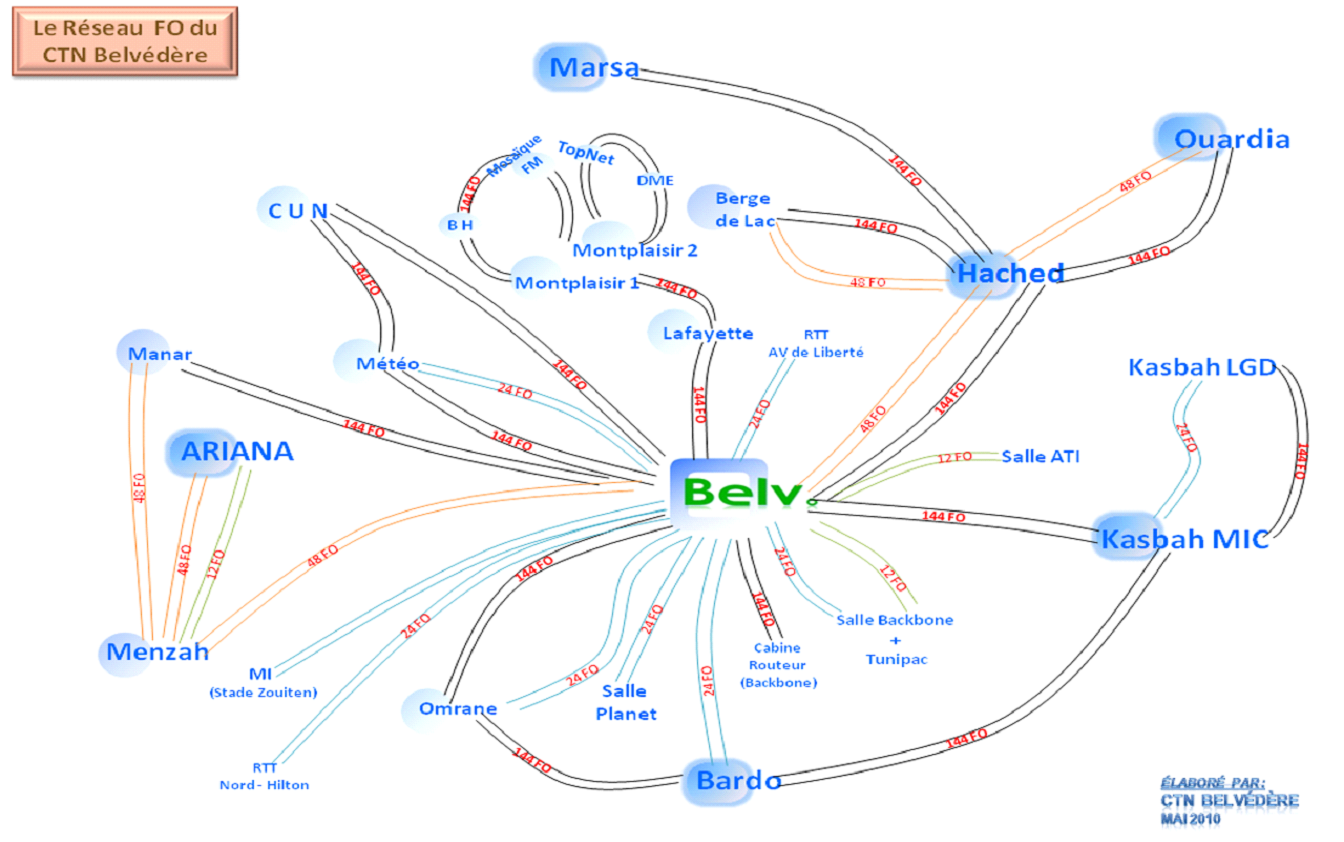
\includegraphics[width=\linewidth]{DTC_Belvedere}
  \caption[DTC Belvedere]{Optic Fibers Map}%\index{Goku il-king}}%
  \label{fig:OFMap}
\end{figure}
We definitely need this tool implemented as a DBMS because traditional .xls files doesn't provide redundancy control, nor does it give different users different profiles and roles, and we know that DBMS's provide all of that and so much more.
\begin{figure}[ht!] % supposedly places it here ...
  \centering
  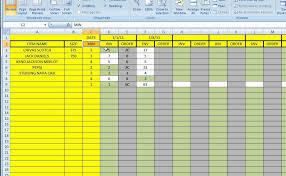
\includegraphics[width=\linewidth]{excel}
  \caption[Excel]{Optic Fibers Map}%\index{Goku il-king}}%
  \label{fig:HowTheyUsedToWork}
\end{figure}
The class diagram is shown in ~\ref{fig:DiagClass1}.
\subsection{Conception}
\begin{figure}[ht!] % supposedly places it here ...
  \centering
  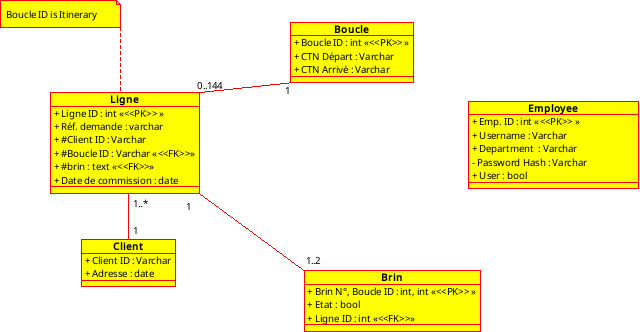
\includegraphics[width=\linewidth]{Class_Diagram}
  \caption[Class Diagram]{Conception}%\index{Goku il-king}}%
  \label{fig:DiagClass1}
\end{figure}
In the Class Diagram and in our project, all revolves around the FiberOptic Ligne, which belongs to a certain Client (company or individual and further details are out of the scope of this work), and is situated on a certain Circuit or 'Boucle' between DTC's, and also which Brin - Boucle pair are attributed to that Ligne along with the status. And then separately, there's an Employee with a status of Admin who has all the permissions on adding, modifying or even deleting Ligne, Client, Boucle, Brin and also other Employees. On the other hand a simple User can only create new Lignes for already existing Clients, on boucles that already exist.
There are 144 Brins per Boucle, and they can have either the status used or unused or under maintenance.
\section{Realisation}%Summary

%\blindtext
Here is a look at the Login screen, the DBMS will automatically recognize which role to grant the Employee. The password is a SHA-256 encrypted and saved in the DBMS.
\begin{figure}[ht!] % supposedly places it here ...
  \centering
  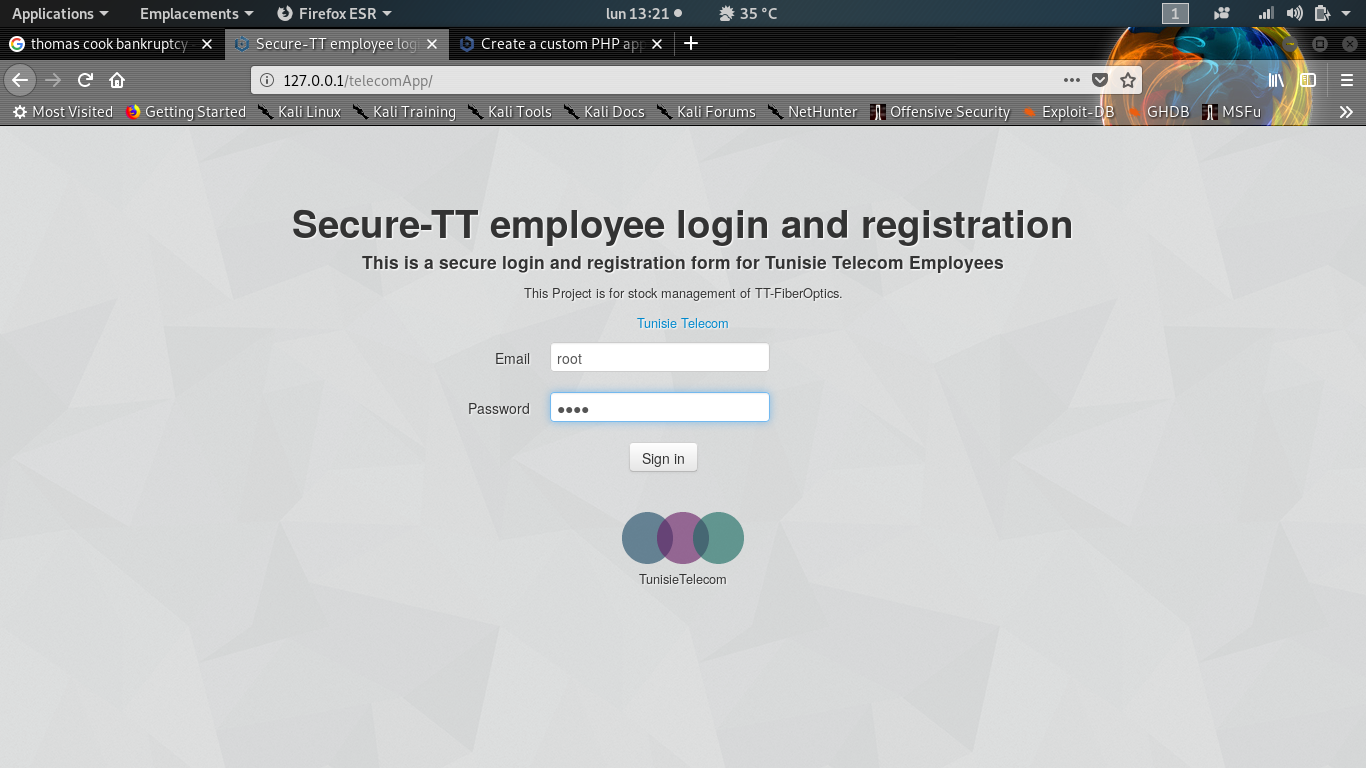
\includegraphics[width=\linewidth]{Login}
  \caption[Login]{Login Screen}%\index{Goku il-king}}%
  \label{fig:Login}
\end{figure}
A User - Employees Dashboard screen is shown below in Figure ~\ref{fig:UserTable}. As you can see, a User can only see things he's allowed to see, and can only modify these things exclusively.
\begin{figure}[ht!] % supposedly places it here ...
  \centering
  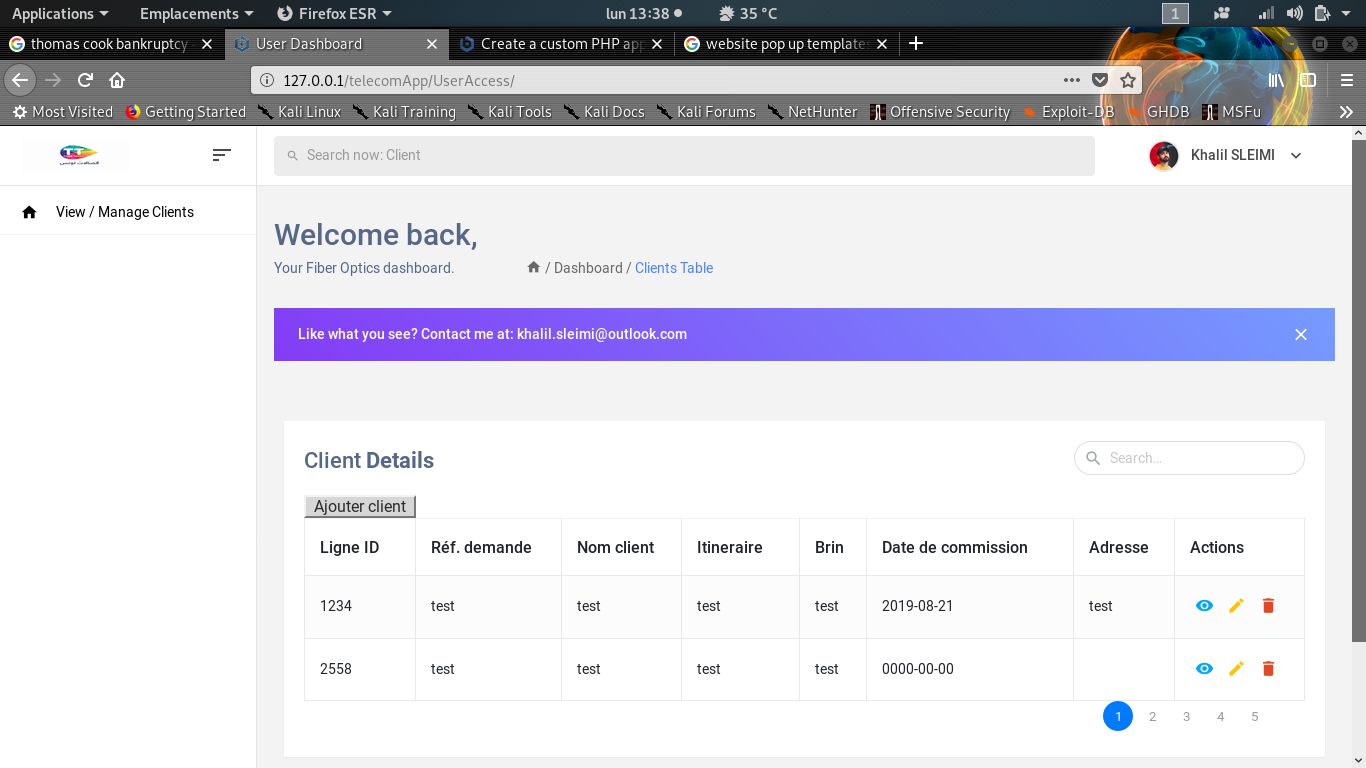
\includegraphics[width=\linewidth]{UserTableau}
  \caption[UserClientsTable]{ User Ligne}%\index{Goku il-king}}%
  \label{fig:UserTable}
\end{figure}
If the Login process recognizes the Employee as being the Admin, the Dashboard will be something like this, He have total control over everything, as is shown on the left, He can manage Clients, or what I presented in the Conception phase above as Ligne (I made the Implementation before the Conception, big mistake, I know), Employees, Boucles and Brins.
\begin{figure}[ht!] % supposedly places it here ...
  \centering
  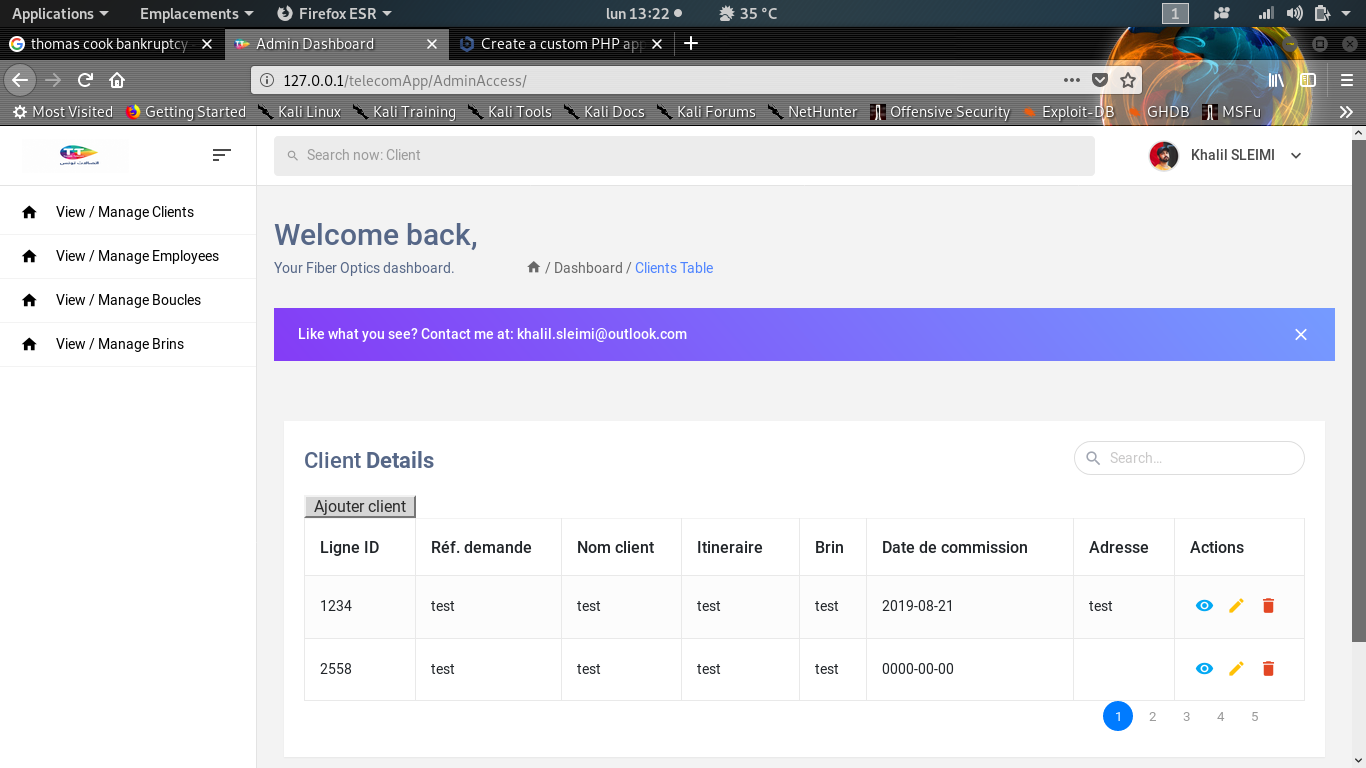
\includegraphics[width=\linewidth]{AdminTableau}
  \caption[AdminClientsTable]{Admin Ligne}%\index{Goku il-king}}%
  \label{fig:AdminClientsTable}
\end{figure}

In this Figure ~\ref{fig:AdminEmployeeTable}, the Admin is allowed to Add, remove or even modify any other Employee, If we'd want it to be some more professional, the Department field will be replaced by a Type field which is either "Admin" or "User". But this was done in less than a month from scratch, and also due to a HDD failure, I don't think I could've done any better - only if I had designed it from the get go and actively used github to back it up - and not forget "git add *" everytime I add some new file.
\begin{figure}[ht!] % supposedly places it here ...
  \centering
  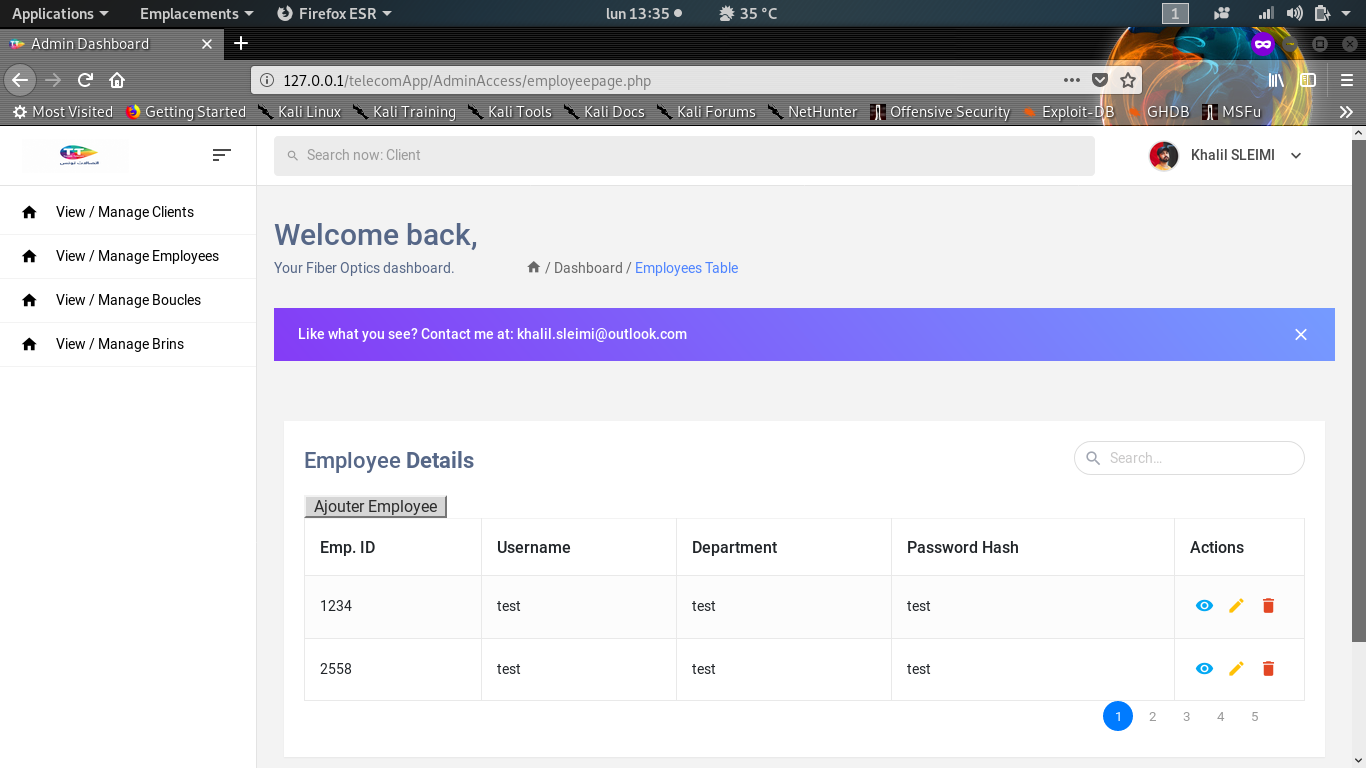
\includegraphics[width=\linewidth]{AdminEmployeeTableau}
  \caption[AdminEmployeeTable]{Admin Employee}%\index{Goku il-king}}%
  \label{fig:AdminEmployeeTable}
\end{figure}

Now, every Ligne is based on a certain Fiber Optic Boucle. This Menu allows the Admin to Manage these Boucles.
\begin{figure}[ht!] % supposedly places it here ...
  \centering
  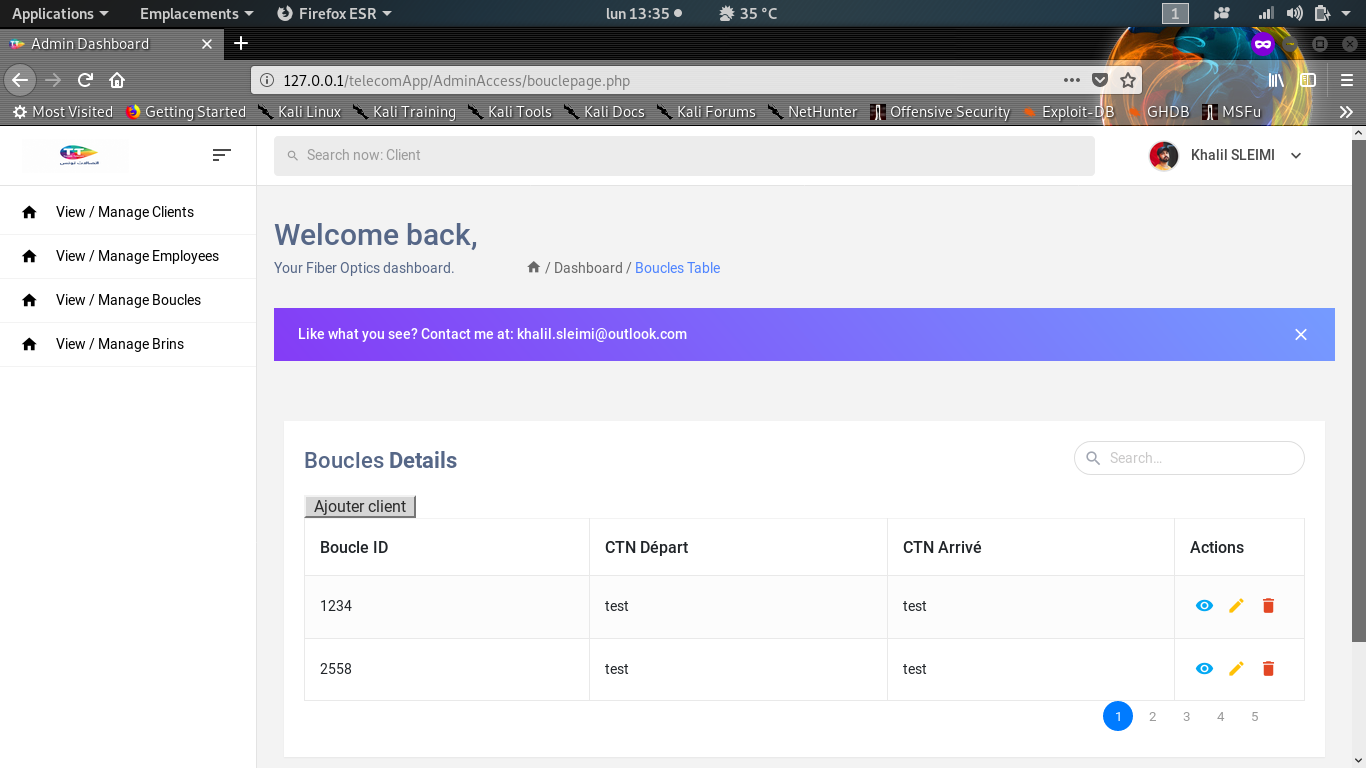
\includegraphics[width=\linewidth]{AdminBouclesTableau}
  \caption[AdminBouclesTable]{Admin Boucles}%\index{Goku il-king}}%
  \label{fig:AdminBouclesTable}
\end{figure}

% \begin{figure}[ht!] % supposedly places it here ...
%   \centering
%   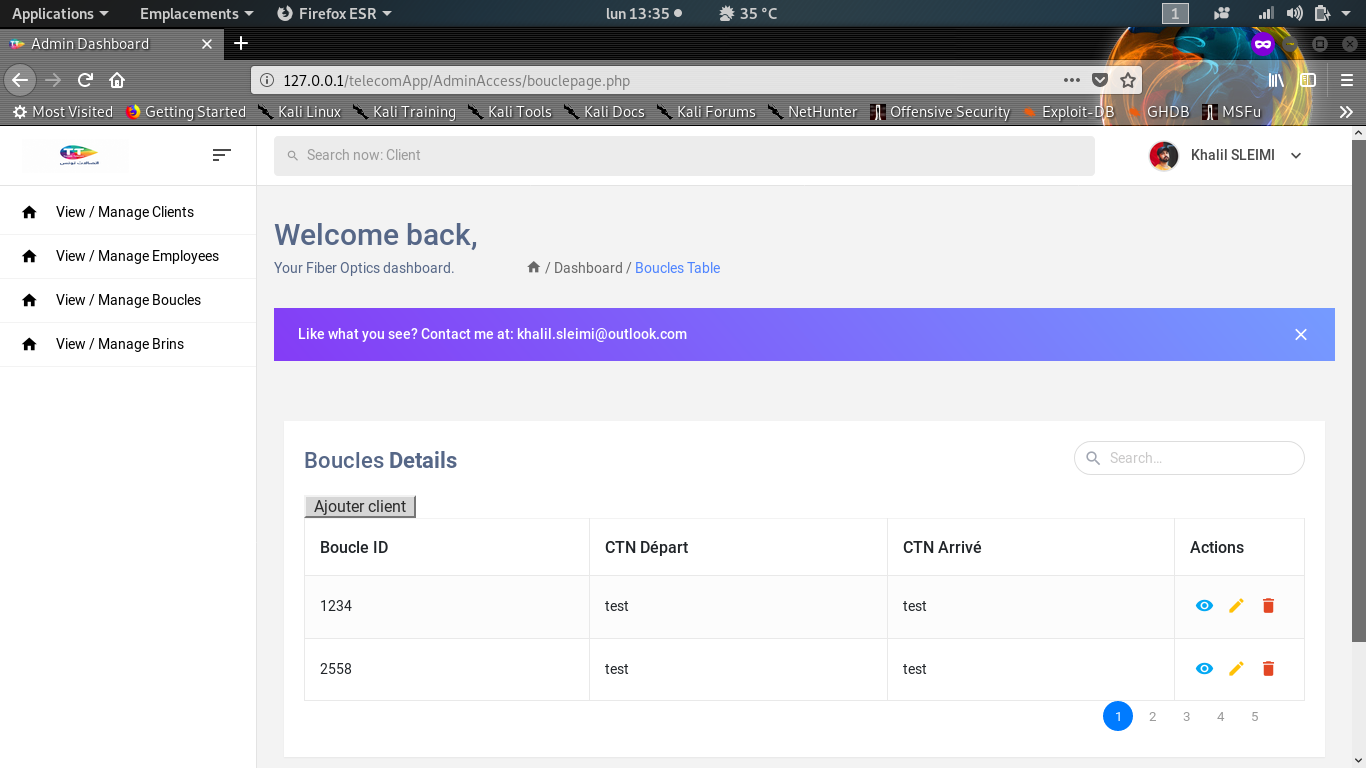
\includegraphics[width=\linewidth]{AdminBouclesTableau}
%   \caption[AdminBrinsTable]{Brins}%\index{Goku il-king}}%
%   \label{fig:AdminBrinsTable}
% \end{figure}

And in this figure is a view of how the pop up for adding and modifying Lignes - Clients is like
\begin{figure}[ht!] % supposedly places it here ...
  \centering
  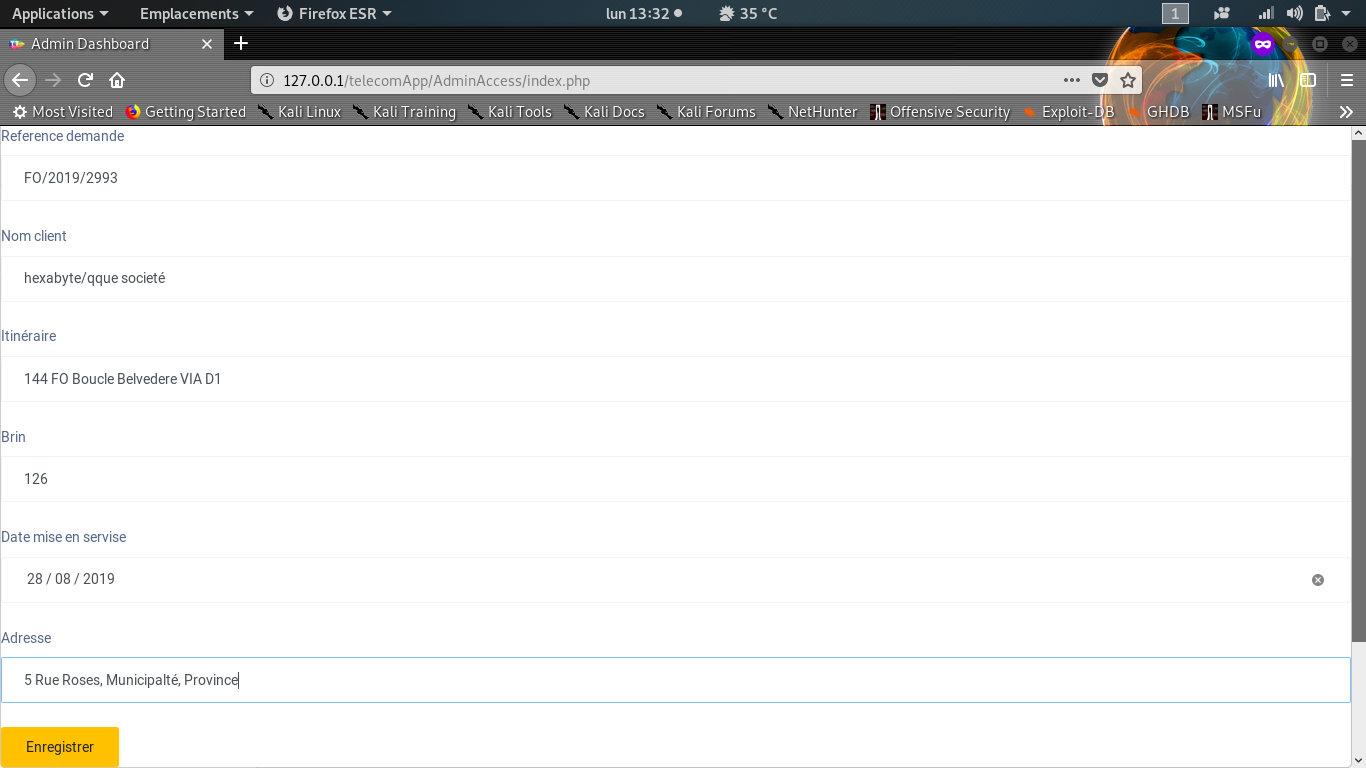
\includegraphics[width=\linewidth]{Popup}
  \caption[Client Pop Up]{Pop Up}%\index{Goku il-king}}%
  \label{fig:Popup}
\end{figure}
